\subsection{Significant data structures}
\subsubsection{The UML Class Diagram}
\begin{sideways}
        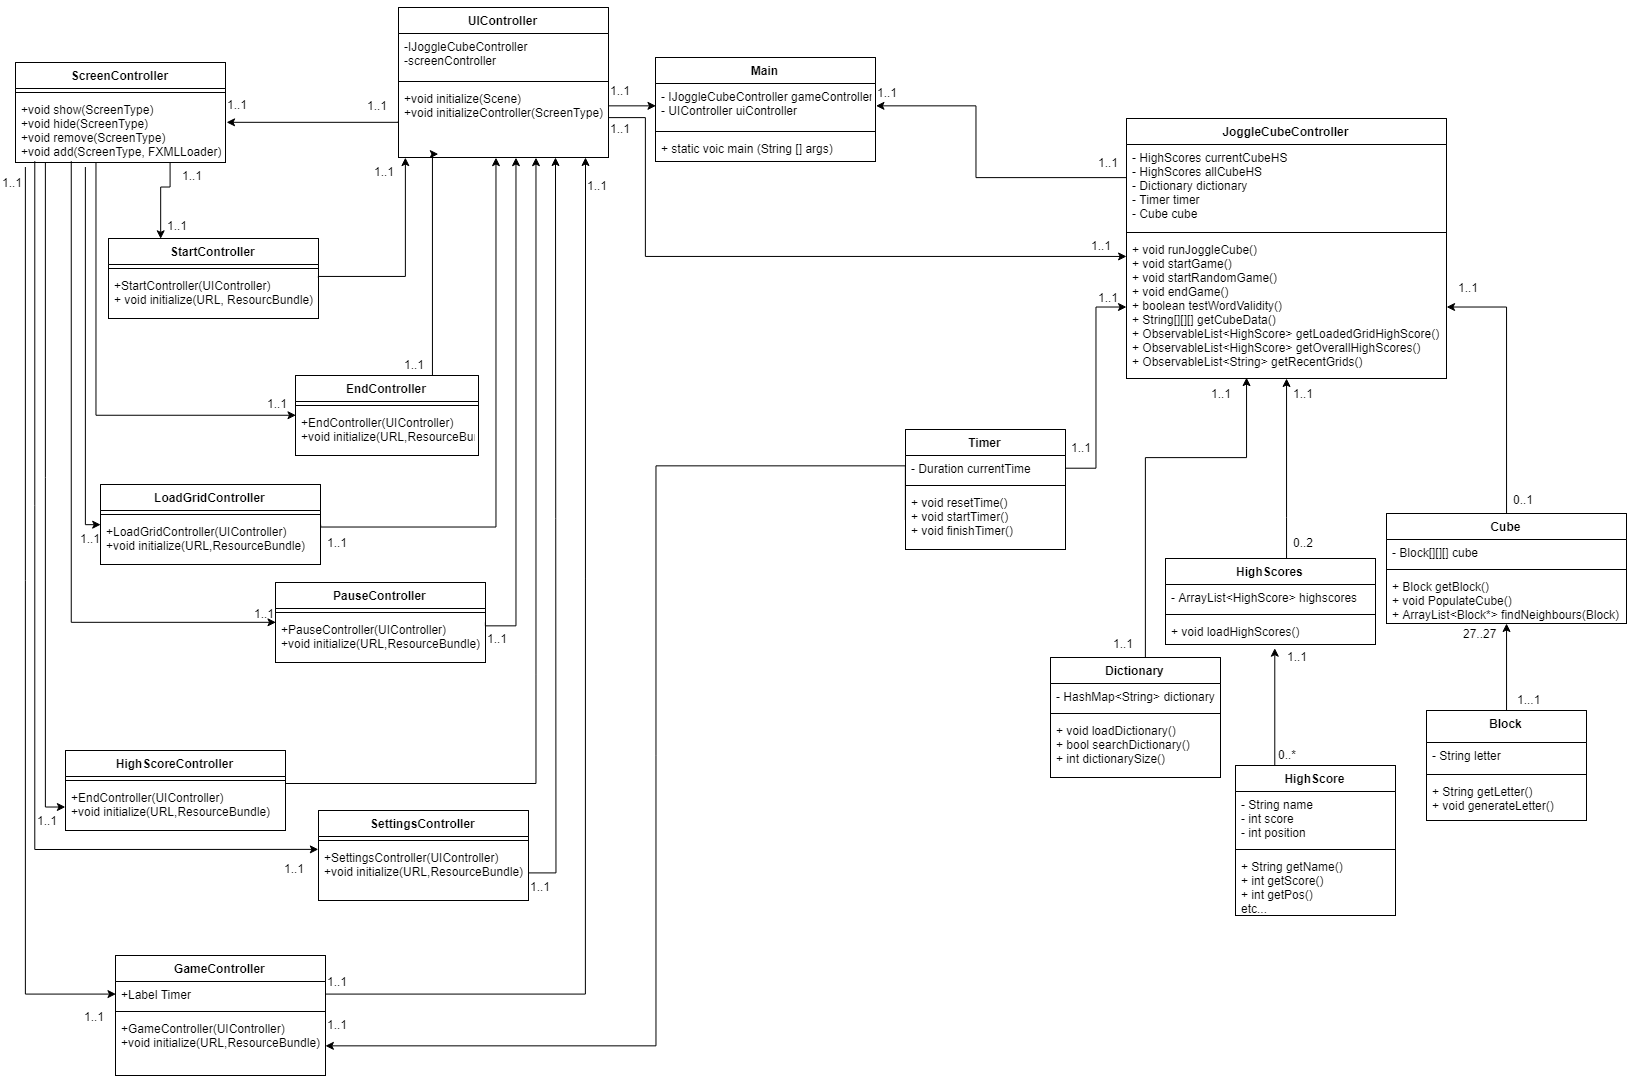
\includegraphics[width=22cm]{Layout_-_drawio_save_ver5_2}
\end{sideways}
        \newpage
    \subsubsection{Object Diagram}
        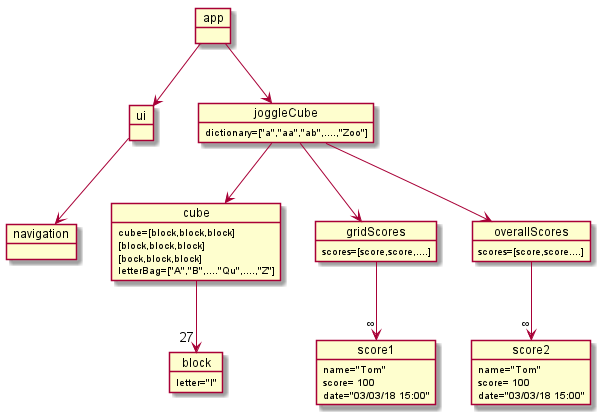
\includegraphics[width=\textwidth]{Cube}
    \subsubsection{Data Persistance}
        \paragraph{Dictionary}
        The way in which Dictionary is kept persistent between program uses is by utilising a text file with no extension. Each dictionary of the program has a very specific layout that must be followed. The document needs to have a word in it for every line, but only one word on each line, if you have 70 words total then you have 70 lines containing one word each. The case of the word doesn't matter as it is handled to take both. The way different dictionaries are loaded is by having the first two characters of the filename be two characters that represent the language e.g. English = en\_dictionary and Welsh = cy\_dictionary.
        
        An example of this can be found in Appendix \ref{DictionaryExample}
        \paragraph{LetterBag}
        The LetterBag needs to be loaded from a specific file with a specific name, the name is parsed similarly to the dictionary in the sense that the naming scheme for English is en\_letters. The letter bag then has one line per letter, the letter is followed by a space then how many times that letter can be "pulled out of the bag" or used in the cube, then it is followed by another space and the score in scrabble not the JoggleCube game (this is applied later). Then the line ends and the next letter happens with the same things after it. e.g. "A 9 1" - is the first line in en\_letters, this also handles Double letters as one so you have Qu represented as "QU 1 8" as a line in the English letter bag. This allows for different languages to be loaded in using the current framework so it's relatively simple to expand the game's language base. The way the LetterBag file is processed by the program has already been discussed earlier in Sections \ref{RandomLetter} and \ref{WordScore}
        
        An example of this can be found in Appendix \ref{LetterBagExample}
        \paragraph{Cube}\label{CubePersistance}
        The Cube is interesting as you need to save the language of that cube to make sure that the correct dictionary and score lists are loaded. The first line of the Cube save files is the language representing by a 2 character string e.g. "en" for English. The next part of the file is the Cube itself, which is 9 lines of 3 characters with spaces between them to represent the grid. This is for visualisation of the cube in the files, with the first character being [0][0][0] and the last being [2][2][2] etc. The Cube then still has its specific high scores to be loaded in which are saved in the Format "Date Time Score Name" with spaces as a delimiter between each value. Further examples of the score can be found in Appendix \ref{HighScoresExample}. The way this file is actually parsed and brought into the program is discussed in Sections: \ref{LoadGrid} and \ref{SaveGrid}
        
        An example of the Cube can be found in Appendix \ref{CubeExample}
        \paragraph{(High) Scores}\label{Scores}
        The (High) Scores part is interesting because it needs to be saved in both Cubes and overAll.highscores and the way this was achieved is with a framework for saving it. The way this is handled for Cubes is described in section \ref{CubePersistance}. The way overAll.highscores is kept persistent is similar to grids but it saves when the program exits or when a grid is finished, and without the grid and language definitions. So it's a long file with one set of HighScores per line with the format "Date time Score Name" e.g. "2018/03/14 15:40 87 player87".
        
        An example of the High Scores can be found in Appendix \ref{HighScoresExample} whilst the way in which individual cubes handle their high scores are discovered in Appendix \ref{CubeExample}